\documentclass[openany]{book}
\usepackage{lmodern}
\usepackage{amssymb,amsmath}
\usepackage{ifxetex,ifluatex}
\usepackage{fixltx2e} % provides \textsubscript
\ifnum 0\ifxetex 1\fi\ifluatex 1\fi=0 % if pdftex
  \usepackage[T1]{fontenc}
  \usepackage[utf8]{inputenc}
\else % if luatex or xelatex
  \ifxetex
    \usepackage{mathspec}
  \else
    \usepackage{fontspec}
  \fi
  \defaultfontfeatures{Ligatures=TeX,Scale=MatchLowercase}
\fi
% use upquote if available, for straight quotes in verbatim environments
\IfFileExists{upquote.sty}{\usepackage{upquote}}{}
% use microtype if available
\IfFileExists{microtype.sty}{%
\usepackage{microtype}
\UseMicrotypeSet[protrusion]{basicmath} % disable protrusion for tt fonts
}{}
\usepackage[margin=1in]{geometry}
\usepackage{hyperref}
\hypersetup{unicode=true,
            pdftitle={R Lab for Statistical Computing},
            pdfborder={0 0 0},
            breaklinks=true}
\urlstyle{same}  % don't use monospace font for urls
\usepackage{natbib}
\bibliographystyle{apalike}
\usepackage{color}
\usepackage{fancyvrb}
\newcommand{\VerbBar}{|}
\newcommand{\VERB}{\Verb[commandchars=\\\{\}]}
\DefineVerbatimEnvironment{Highlighting}{Verbatim}{commandchars=\\\{\}}
% Add ',fontsize=\small' for more characters per line
\usepackage{framed}
\definecolor{shadecolor}{RGB}{248,248,248}
\newenvironment{Shaded}{\begin{snugshade}}{\end{snugshade}}
\newcommand{\AlertTok}[1]{\textcolor[rgb]{0.94,0.16,0.16}{#1}}
\newcommand{\AnnotationTok}[1]{\textcolor[rgb]{0.56,0.35,0.01}{\textbf{\textit{#1}}}}
\newcommand{\AttributeTok}[1]{\textcolor[rgb]{0.77,0.63,0.00}{#1}}
\newcommand{\BaseNTok}[1]{\textcolor[rgb]{0.00,0.00,0.81}{#1}}
\newcommand{\BuiltInTok}[1]{#1}
\newcommand{\CharTok}[1]{\textcolor[rgb]{0.31,0.60,0.02}{#1}}
\newcommand{\CommentTok}[1]{\textcolor[rgb]{0.56,0.35,0.01}{\textit{#1}}}
\newcommand{\CommentVarTok}[1]{\textcolor[rgb]{0.56,0.35,0.01}{\textbf{\textit{#1}}}}
\newcommand{\ConstantTok}[1]{\textcolor[rgb]{0.00,0.00,0.00}{#1}}
\newcommand{\ControlFlowTok}[1]{\textcolor[rgb]{0.13,0.29,0.53}{\textbf{#1}}}
\newcommand{\DataTypeTok}[1]{\textcolor[rgb]{0.13,0.29,0.53}{#1}}
\newcommand{\DecValTok}[1]{\textcolor[rgb]{0.00,0.00,0.81}{#1}}
\newcommand{\DocumentationTok}[1]{\textcolor[rgb]{0.56,0.35,0.01}{\textbf{\textit{#1}}}}
\newcommand{\ErrorTok}[1]{\textcolor[rgb]{0.64,0.00,0.00}{\textbf{#1}}}
\newcommand{\ExtensionTok}[1]{#1}
\newcommand{\FloatTok}[1]{\textcolor[rgb]{0.00,0.00,0.81}{#1}}
\newcommand{\FunctionTok}[1]{\textcolor[rgb]{0.00,0.00,0.00}{#1}}
\newcommand{\ImportTok}[1]{#1}
\newcommand{\InformationTok}[1]{\textcolor[rgb]{0.56,0.35,0.01}{\textbf{\textit{#1}}}}
\newcommand{\KeywordTok}[1]{\textcolor[rgb]{0.13,0.29,0.53}{\textbf{#1}}}
\newcommand{\NormalTok}[1]{#1}
\newcommand{\OperatorTok}[1]{\textcolor[rgb]{0.81,0.36,0.00}{\textbf{#1}}}
\newcommand{\OtherTok}[1]{\textcolor[rgb]{0.56,0.35,0.01}{#1}}
\newcommand{\PreprocessorTok}[1]{\textcolor[rgb]{0.56,0.35,0.01}{\textit{#1}}}
\newcommand{\RegionMarkerTok}[1]{#1}
\newcommand{\SpecialCharTok}[1]{\textcolor[rgb]{0.00,0.00,0.00}{#1}}
\newcommand{\SpecialStringTok}[1]{\textcolor[rgb]{0.31,0.60,0.02}{#1}}
\newcommand{\StringTok}[1]{\textcolor[rgb]{0.31,0.60,0.02}{#1}}
\newcommand{\VariableTok}[1]{\textcolor[rgb]{0.00,0.00,0.00}{#1}}
\newcommand{\VerbatimStringTok}[1]{\textcolor[rgb]{0.31,0.60,0.02}{#1}}
\newcommand{\WarningTok}[1]{\textcolor[rgb]{0.56,0.35,0.01}{\textbf{\textit{#1}}}}
\usepackage{longtable,booktabs}
\usepackage{graphicx,grffile}
\makeatletter
\def\maxwidth{\ifdim\Gin@nat@width>\linewidth\linewidth\else\Gin@nat@width\fi}
\def\maxheight{\ifdim\Gin@nat@height>\textheight\textheight\else\Gin@nat@height\fi}
\makeatother
% Scale images if necessary, so that they will not overflow the page
% margins by default, and it is still possible to overwrite the defaults
% using explicit options in \includegraphics[width, height, ...]{}
\setkeys{Gin}{width=\maxwidth,height=\maxheight,keepaspectratio}
\IfFileExists{parskip.sty}{%
\usepackage{parskip}
}{% else
\setlength{\parindent}{0pt}
\setlength{\parskip}{6pt plus 2pt minus 1pt}
}
\setlength{\emergencystretch}{3em}  % prevent overfull lines
\providecommand{\tightlist}{%
  \setlength{\itemsep}{0pt}\setlength{\parskip}{0pt}}
\setcounter{secnumdepth}{5}
% Redefines (sub)paragraphs to behave more like sections
\ifx\paragraph\undefined\else
\let\oldparagraph\paragraph
\renewcommand{\paragraph}[1]{\oldparagraph{#1}\mbox{}}
\fi
\ifx\subparagraph\undefined\else
\let\oldsubparagraph\subparagraph
\renewcommand{\subparagraph}[1]{\oldsubparagraph{#1}\mbox{}}
\fi

%%% Use protect on footnotes to avoid problems with footnotes in titles
\let\rmarkdownfootnote\footnote%
\def\footnote{\protect\rmarkdownfootnote}

%%% Change title format to be more compact
\usepackage{titling}

% Create subtitle command for use in maketitle
\providecommand{\subtitle}[1]{
  \posttitle{
    \begin{center}\large#1\end{center}
    }
}

\setlength{\droptitle}{-2em}

  \title{R Lab for Statistical Computing}
    \pretitle{\vspace{\droptitle}\centering\huge}
  \posttitle{\par}
    \author{Young-geun Kim\\
Department of Statistics, SKKU\\
\href{mailto: dudrms33@g.skku.edu}{dudrms33@g.skku.edu}}
    \preauthor{\centering\large\emph}
  \postauthor{\par}
      \predate{\centering\large\emph}
  \postdate{\par}
    \date{2019-04-07}

\usepackage{booktabs}
\usepackage{float}
\usepackage{pdfpages}

\newcommand{\iid}{\stackrel{iid}{\sim}}
\newcommand{\indep}{\stackrel{indep}{\sim}}
\newcommand{\hsim}{\stackrel{H_0}{\sim}}
\newcommand{\ind}{\perp\!\!\!\perp}
\newcommand{\R}{\mathbb{R}}
\DeclareMathOperator*{\argmin}{argmin}

\let\oldmaketitle\maketitle
\AtBeginDocument{\let\maketitle\relax}

\usepackage{amsthm}
\newtheorem{theorem}{Theorem}[chapter]
\newtheorem{lemma}{Lemma}[chapter]
\newtheorem{corollary}{Corollary}[chapter]
\newtheorem{proposition}{Proposition}[chapter]
\newtheorem{conjecture}{Conjecture}[chapter]
\theoremstyle{definition}
\newtheorem{definition}{Definition}[chapter]
\theoremstyle{definition}
\newtheorem{example}{Example}[chapter]
\theoremstyle{definition}
\newtheorem{exercise}{Exercise}[chapter]
\theoremstyle{remark}
\newtheorem*{remark}{Remark}
\newtheorem*{solution}{Solution}
\let\BeginKnitrBlock\begin \let\EndKnitrBlock\end
\begin{document}
\maketitle

\begin{titlepage}
  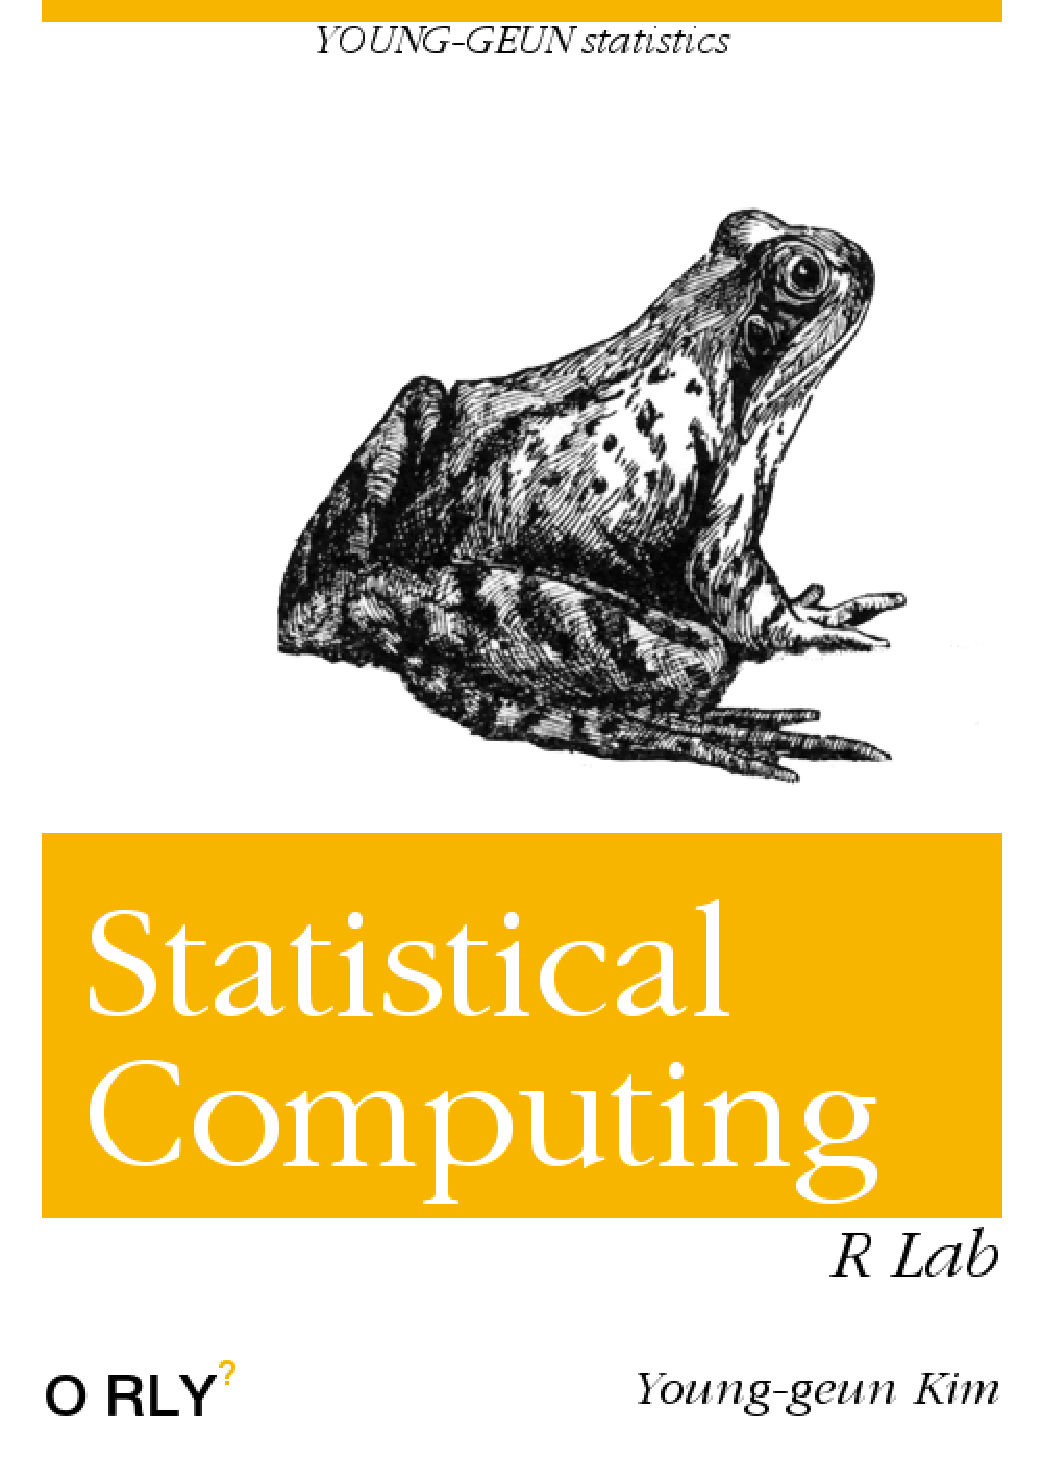
\includepdf{cover.pdf}
\end{titlepage}

\let\maketitle\oldmaketitle
\maketitle

{
\setcounter{tocdepth}{1}
\tableofcontents
}
\hypertarget{welcome}{%
\chapter*{Welcome}\label{welcome}}
\addcontentsline{toc}{chapter}{Welcome}

Statistical computing mainly treats useful simulation methods.

\hypertarget{statistical-computing}{%
\section*{Statistical Computing}\label{statistical-computing}}
\addcontentsline{toc}{section}{Statistical Computing}

We first look at \emph{random generation} methods. Lots of simulation methods are built based on this random numbers.

\hypertarget{sampling-from-a-fininte-population}{%
\subsection*{Sampling from a fininte population}\label{sampling-from-a-fininte-population}}
\addcontentsline{toc}{subsection}{Sampling from a fininte population}

Generating random numbers is like sampling. From finite population, we can sample data with or without replacement. For example of sampling with replacement, we toss coins 10 times.

\begin{Shaded}
\begin{Highlighting}[]
\KeywordTok{sample}\NormalTok{(}\DecValTok{0}\OperatorTok{:}\DecValTok{1}\NormalTok{, }\DataTypeTok{size =} \DecValTok{10}\NormalTok{, }\DataTypeTok{replace =} \OtherTok{TRUE}\NormalTok{)}
\NormalTok{ [}\DecValTok{1}\NormalTok{] }\DecValTok{1} \DecValTok{0} \DecValTok{0} \DecValTok{1} \DecValTok{0} \DecValTok{1} \DecValTok{1} \DecValTok{0} \DecValTok{1} \DecValTok{1}
\end{Highlighting}
\end{Shaded}

Sampling without replacement: Choose some lottery numbers which consist of 1 to 100.

\begin{Shaded}
\begin{Highlighting}[]
\KeywordTok{sample}\NormalTok{(}\DecValTok{1}\OperatorTok{:}\DecValTok{100}\NormalTok{, }\DataTypeTok{size =} \DecValTok{6}\NormalTok{, }\DataTypeTok{replace =} \OtherTok{FALSE}\NormalTok{)}
\NormalTok{[}\DecValTok{1}\NormalTok{] }\DecValTok{61} \DecValTok{83} \DecValTok{50} \DecValTok{74} \DecValTok{34} \DecValTok{35}
\end{Highlighting}
\end{Shaded}

\hypertarget{random-generators-of-common-probability-distributions}{%
\subsection*{Random generators of common probability distributions}\label{random-generators-of-common-probability-distributions}}
\addcontentsline{toc}{subsection}{Random generators of common probability distributions}

\texttt{R} provides some functions which generate random numbers following famous distributions. Although we will learn some skills generating these numbers in basis levels, these functions do the same thing more elegantly.

\begin{Shaded}
\begin{Highlighting}[]
\KeywordTok{gg_curve}\NormalTok{(dbeta, }\DataTypeTok{from =} \DecValTok{0}\NormalTok{, }\DataTypeTok{to =} \DecValTok{1}\NormalTok{, }\DataTypeTok{args =} \KeywordTok{list}\NormalTok{(}\DataTypeTok{shape1 =} \DecValTok{3}\NormalTok{, }\DataTypeTok{shape2 =} \DecValTok{2}\NormalTok{)) }\OperatorTok{+}
\StringTok{  }\KeywordTok{geom_histogram}\NormalTok{(}
    \DataTypeTok{data =} \KeywordTok{tibble}\NormalTok{(}
      \DataTypeTok{rand =} \KeywordTok{rbeta}\NormalTok{(}\DecValTok{1000}\NormalTok{, }\DecValTok{3}\NormalTok{, }\DecValTok{2}\NormalTok{),}
      \DataTypeTok{idx =} \KeywordTok{seq}\NormalTok{(}\DecValTok{0}\NormalTok{, }\DecValTok{1}\NormalTok{, }\DataTypeTok{length.out =} \DecValTok{1000}\NormalTok{)}
\NormalTok{    ),}
    \KeywordTok{aes}\NormalTok{(}\DataTypeTok{x =}\NormalTok{ rand, }\DataTypeTok{y =}\NormalTok{ ..density..),}
    \DataTypeTok{position =} \StringTok{"identity"}\NormalTok{,}
    \DataTypeTok{bins =} \DecValTok{30}\NormalTok{,}
    \DataTypeTok{alpha =} \FloatTok{.45}\NormalTok{,}
    \DataTypeTok{fill =} \KeywordTok{gg_hcl}\NormalTok{(}\DecValTok{1}\NormalTok{)}
\NormalTok{  )}
\end{Highlighting}
\end{Shaded}

\begin{figure}[H]

{\centering 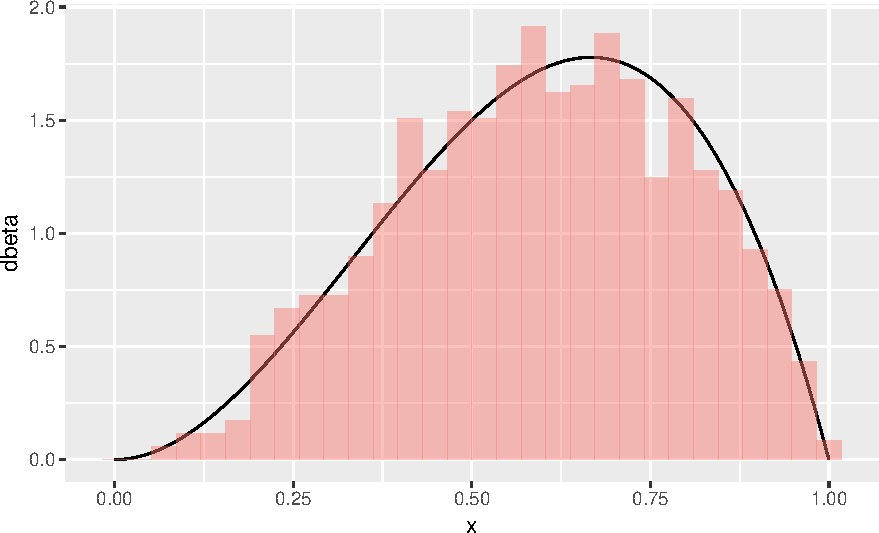
\includegraphics[width=0.7\linewidth]{statistical-computing_files/figure-latex/dbrb-1} 

}

\caption{Beta(3,2) random numbers}\label{fig:dbrb}
\end{figure}

Figure \ref{fig:dbrb} shows that \texttt{rbeta()} function generate random numbers very well. Histogram is of the random number, and the curve is the true beta distribution.

\hypertarget{rvar}{%
\chapter{Methods for Generating Random Variables}\label{rvar}}

\hypertarget{introduction}{%
\section{Introduction}\label{introduction}}

Most of the methods so-called \emph{computational statistics} requires generation of random variables from specified probability distribution. In hand, we can spin wheels, roll a dice, or shuffle cards. The results are chosen randomly. However, we want the same things with computer. Here, \texttt{r}. As we know, computer cannot generate complete uniform random numbers. Instead, we generate \textbf{pseudo-random} numbers.

\hypertarget{pseudo-random-numbers}{%
\section{Pseudo-random Numbers}\label{pseudo-random-numbers}}

\BeginKnitrBlock{definition}[Pseudo-random numbers]
\protect\hypertarget{def:unnamed-chunk-5}{}{\label{def:unnamed-chunk-5} \iffalse (Pseudo-random numbers) \fi{} }Sequence of values generated deterministically which have all the appearances of being independent \(unif(0, 1)\) random variables, i.e.

\[x_1, x_2, \ldots, x_n \stackrel{iid}{\sim} unif(0, 1)\]
\EndKnitrBlock{definition}

\begin{itemize}
\tightlist
\item
  behave \emph{as if} following \(unif(0, 1)\)
\item
  typically generated from an \emph{initial seed}
\end{itemize}

\hypertarget{linear-congruential-generator}{%
\subsection{Linear congruential generator}\label{linear-congruential-generator}}

Let \(x_0, x_1, \ldots \in \mathbb{Z}_{+}\).

\begin{enumerate}
\def\labelenumi{\arabic{enumi}.}
\tightlist
\item
  Set \(x_0\) as initial seed.
\item
  Generate \(x_n, n = 1, 2, \ldots\) recursively:

  \begin{enumerate}
  \def\labelenumii{\alph{enumii}.}
  \tightlist
  \item
    \(x_n = (a x_{n - 1} + c) \mod m\)
  \item
    where \(a, c \in \mathbb{Z}_{+}, m: \text{modulus}\)
  \end{enumerate}
\item
  Compute \(u_n = \frac{x_n}{m} \in (0, 1)\)
\end{enumerate}

Then \(u_1, u_2, \ldots \sim unif(0, 1)\)

\begin{Shaded}
\begin{Highlighting}[]
\NormalTok{lcg <-}\StringTok{ }\ControlFlowTok{function}\NormalTok{(n, seed, a, b, m) \{}
\NormalTok{  x <-}\StringTok{ }\KeywordTok{rep}\NormalTok{(seed, n }\OperatorTok{+}\StringTok{ }\DecValTok{1}\NormalTok{)}
  \ControlFlowTok{for}\NormalTok{ (i }\ControlFlowTok{in} \DecValTok{1}\OperatorTok{:}\NormalTok{n) \{}
\NormalTok{    x[i }\OperatorTok{+}\StringTok{ }\DecValTok{1}\NormalTok{] <-}\StringTok{ }\NormalTok{(a }\OperatorTok{*}\StringTok{ }\NormalTok{x[i] }\OperatorTok{+}\StringTok{ }\NormalTok{b) }\OperatorTok\StringTok{ }\NormalTok{m}
\NormalTok{  \}}
\NormalTok{  x[}\OperatorTok{-}\DecValTok{1}\NormalTok{] }\OperatorTok{/}\StringTok{ }\NormalTok{m}
\NormalTok{\}}
\end{Highlighting}
\end{Shaded}

\begin{Shaded}
\begin{Highlighting}[]
\KeywordTok{tibble}\NormalTok{(}
  \DataTypeTok{x =} \KeywordTok{lcg}\NormalTok{(}\DecValTok{1000}\NormalTok{, }\DecValTok{0}\NormalTok{, }\DecValTok{1664525}\NormalTok{, }\DecValTok{1013904223}\NormalTok{, }\DecValTok{2}\OperatorTok{^}\DecValTok{32}\NormalTok{)}
\NormalTok{) }\OperatorTok\StringTok{ }
\StringTok{  }\KeywordTok{ggplot}\NormalTok{(}\KeywordTok{aes}\NormalTok{(}\DataTypeTok{x =}\NormalTok{ x)) }\OperatorTok{+}
\StringTok{  }\KeywordTok{geom_histogram}\NormalTok{(}\KeywordTok{aes}\NormalTok{(}\DataTypeTok{y =}\NormalTok{ ..density..), }\DataTypeTok{bins =} \DecValTok{30}\NormalTok{, }\DataTypeTok{col =} \KeywordTok{gg_hcl}\NormalTok{(}\DecValTok{1}\NormalTok{))}
\end{Highlighting}
\end{Shaded}

\begin{center}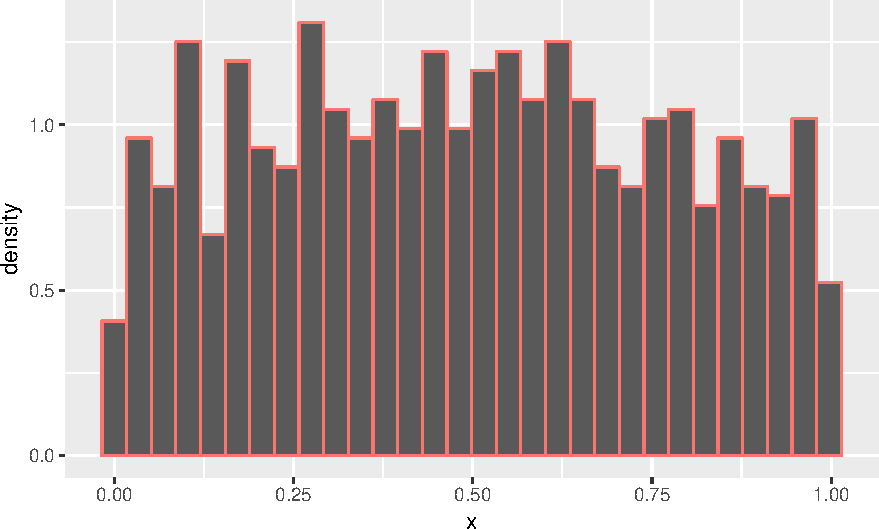
\includegraphics[width=0.7\linewidth]{statistical-computing_files/figure-latex/unnamed-chunk-7-1} \end{center}

\hypertarget{multiplicative-congruential-generator}{%
\subsection{Multiplicative congruential generator}\label{multiplicative-congruential-generator}}

As we can expect from its name, this is congruential generator with \(c = 0\).

\begin{enumerate}
\def\labelenumi{\arabic{enumi}.}
\tightlist
\item
  Set \(x_0\) as initial seed.
\item
  Generate \(x_n, n = 1, 2, \ldots\) recursively:

  \begin{enumerate}
  \def\labelenumii{\alph{enumii}.}
  \tightlist
  \item
    \(x_n = a x_{n - 1} \mod m\)
  \item
    where \(a \in \mathbb{Z}_{+}, m: \text{modulus}\)
  \end{enumerate}
\item
  Compute \(u_n = \frac{x_n}{m} \in (0, 1)\)
\end{enumerate}

Then \(u_1, u_2, \ldots \sim unif(0, 1)\)

We just set \texttt{b\ =\ 0} in our \texttt{lcg()} function. The \textbf{seed must not be zero}.

\begin{Shaded}
\begin{Highlighting}[]
\KeywordTok{tibble}\NormalTok{(}
  \DataTypeTok{x =} \KeywordTok{lcg}\NormalTok{(}\DecValTok{1000}\NormalTok{, }\DecValTok{5}\NormalTok{, }\DecValTok{1664525}\NormalTok{, }\DecValTok{0}\NormalTok{, }\DecValTok{2}\OperatorTok{^}\DecValTok{32}\NormalTok{)}
\NormalTok{) }\OperatorTok\StringTok{ }
\StringTok{  }\KeywordTok{ggplot}\NormalTok{(}\KeywordTok{aes}\NormalTok{(}\DataTypeTok{x =}\NormalTok{ x)) }\OperatorTok{+}
\StringTok{  }\KeywordTok{geom_histogram}\NormalTok{(}\KeywordTok{aes}\NormalTok{(}\DataTypeTok{y =}\NormalTok{ ..density..), }\DataTypeTok{bins =} \DecValTok{30}\NormalTok{, }\DataTypeTok{col =} \KeywordTok{gg_hcl}\NormalTok{(}\DecValTok{1}\NormalTok{))}
\end{Highlighting}
\end{Shaded}

\begin{center}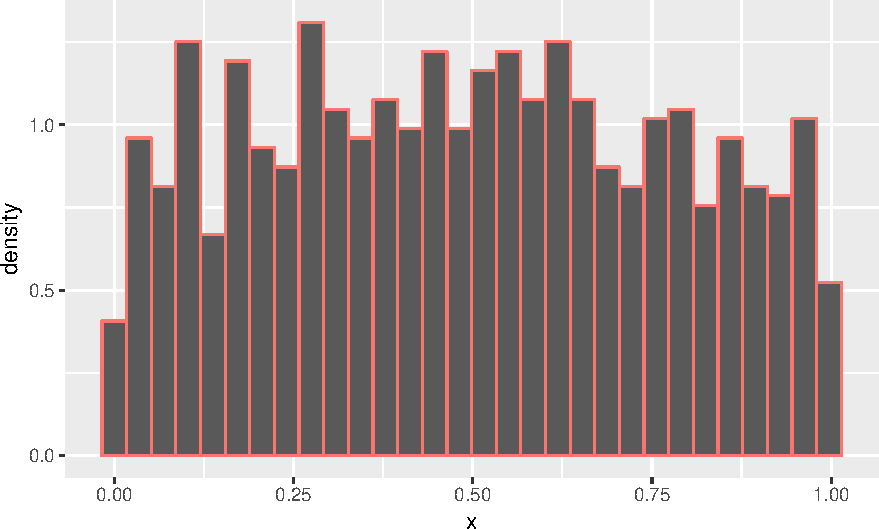
\includegraphics[width=0.7\linewidth]{statistical-computing_files/figure-latex/unnamed-chunk-8-1} \end{center}

\hypertarget{cycle}{%
\subsection{Cycle}\label{cycle}}

Generate LCG \(n = 32\) with \(a = 1\), \(c = 1\), and \(m = 16\) from the seed \(x_0 = 0\).

\begin{Shaded}
\begin{Highlighting}[]
\KeywordTok{lcg}\NormalTok{(}\DecValTok{32}\NormalTok{, }\DecValTok{0}\NormalTok{, }\DecValTok{1}\NormalTok{, }\DecValTok{1}\NormalTok{, }\DecValTok{16}\NormalTok{)}
\NormalTok{ [}\DecValTok{1}\NormalTok{] }\FloatTok{0.0625} \FloatTok{0.1250} \FloatTok{0.1875} \FloatTok{0.2500} \FloatTok{0.3125} \FloatTok{0.3750} \FloatTok{0.4375} \FloatTok{0.5000} \FloatTok{0.5625} \FloatTok{0.6250}
\NormalTok{[}\DecValTok{11}\NormalTok{] }\FloatTok{0.6875} \FloatTok{0.7500} \FloatTok{0.8125} \FloatTok{0.8750} \FloatTok{0.9375} \FloatTok{0.0000} \FloatTok{0.0625} \FloatTok{0.1250} \FloatTok{0.1875} \FloatTok{0.2500}
\NormalTok{[}\DecValTok{21}\NormalTok{] }\FloatTok{0.3125} \FloatTok{0.3750} \FloatTok{0.4375} \FloatTok{0.5000} \FloatTok{0.5625} \FloatTok{0.6250} \FloatTok{0.6875} \FloatTok{0.7500} \FloatTok{0.8125} \FloatTok{0.8750}
\NormalTok{[}\DecValTok{31}\NormalTok{] }\FloatTok{0.9375} \FloatTok{0.0000}
\end{Highlighting}
\end{Shaded}

Observe that we have the cycle after \(m\)-th number. Against this problem, we give different seed from every \((im + 1)\)th random number.

\hypertarget{the-inverse-transform-method}{%
\section{The Inverse Transform Method}\label{the-inverse-transform-method}}

\BeginKnitrBlock{definition}[Inverse of CDF]
\protect\hypertarget{def:icdf}{}{\label{def:icdf} \iffalse (Inverse of CDF) \fi{} }Since some cdf \(F_X\) is not strictly increasing, we difine \(F_X^{-1}(y)\) for \(0 < y < 1\) by

\[F_{X}^{-1}(y) := inf \{ x : F_X(x) \ge y \}\]
\EndKnitrBlock{definition}

Using this definition, we can get the following theorem.

\BeginKnitrBlock{theorem}[Probability Integral Transformation]
\protect\hypertarget{thm:probint}{}{\label{thm:probint} \iffalse (Probability Integral Transformation) \fi{} }If \(X\) is a continuous random variable with cdf \(F_(x)\), then
\[U \equiv F_X(X) \sim unif(0, 1)\]
\EndKnitrBlock{theorem}

\BeginKnitrBlock{proof}[Probability Integral Transformation]
\iffalse{} {Proof (Probability Integral Transformation). } \fi{}Let \(U \sim unif(0, 1)\). Then

\begin{equation*}
  \begin{split}
    P(F_X^{-1}(U) \le x) & = P(\inf\{t : F_X(t) = U \} \le x) \\
    & = P(U \le F_X(x)) \\
    & = F_U(F_X(x)) \\
    & = F_X(x)
  \end{split}
\end{equation*}
\EndKnitrBlock{proof}

Thus, to generate \(n\) random variables \(\sim F_X\),

\begin{enumerate}
\def\labelenumi{\arabic{enumi}.}
\tightlist
\item
  form of \(F_X^{-1}(u)\)
\item
  For each \(i = 1, 2, \ldots, n\):

  \begin{enumerate}
  \def\labelenumii{\alph{enumii}.}
  \tightlist
  \item
    Generate \(u_i \sim unif(0, 1)\)
  \item
    \(x_i = F_X^{-1}(u_i)\)
  \end{enumerate}
\end{enumerate}

Collect \(x_1, x_2, \ldots, x_n \stackrel{iid}{\sim} F_X\).

\hypertarget{continuous-case}{%
\subsection{Continuous case}\label{continuous-case}}

Denote that the \emph{probability integral transformation} holds for a continuous variable. When generating continuous random variable, applying above algorithm might work.

\BeginKnitrBlock{example}[Exponential distribution]
\protect\hypertarget{exm:expon}{}{\label{exm:expon} \iffalse (Exponential distribution) \fi{} }If \(X \sim Exp(\lambda)\), then \(F_X(x) = 1 - e^{-\lambda x}\). We can derive the inverse function of cdf
\[F_X^{-1}(u) = \frac{1}{\lambda}\ln(1 - u)\]
\EndKnitrBlock{example}

Note that

\[U \sim unif(0, 1) \Leftrightarrow 1 - U \sim unif(0, 1)\]

Then we just can use \(U\) instead of \(1 - U\).

\begin{Shaded}
\begin{Highlighting}[]
\NormalTok{inv_exp <-}\StringTok{ }\ControlFlowTok{function}\NormalTok{(n, lambda) \{}
  \OperatorTok{-}\KeywordTok{log}\NormalTok{(}\KeywordTok{runif}\NormalTok{(n)) }\OperatorTok{/}\StringTok{ }\NormalTok{lambda}
\NormalTok{\}}
\end{Highlighting}
\end{Shaded}

If we generate \(x_1, \ldots, x_{500} \sim Exp(\lambda = 1)\),

\begin{Shaded}
\begin{Highlighting}[]
\KeywordTok{gg_curve}\NormalTok{(dexp, }\DataTypeTok{from =} \DecValTok{0}\NormalTok{, }\DataTypeTok{to =} \DecValTok{10}\NormalTok{) }\OperatorTok{+}
\StringTok{  }\KeywordTok{geom_histogram}\NormalTok{(}
    \DataTypeTok{data =} \KeywordTok{tibble}\NormalTok{(}\DataTypeTok{x =} \KeywordTok{inv_exp}\NormalTok{(}\DecValTok{500}\NormalTok{, }\DataTypeTok{lambda =} \DecValTok{1}\NormalTok{)),}
    \KeywordTok{aes}\NormalTok{(}\DataTypeTok{x =}\NormalTok{ x, }\DataTypeTok{y =}\NormalTok{ ..density..),}
    \DataTypeTok{bins =} \DecValTok{30}\NormalTok{,}
    \DataTypeTok{fill =} \KeywordTok{gg_hcl}\NormalTok{(}\DecValTok{1}\NormalTok{),}
    \DataTypeTok{alpha =} \FloatTok{.5}
\NormalTok{  )}
\end{Highlighting}
\end{Shaded}

\begin{figure}[H]

{\centering 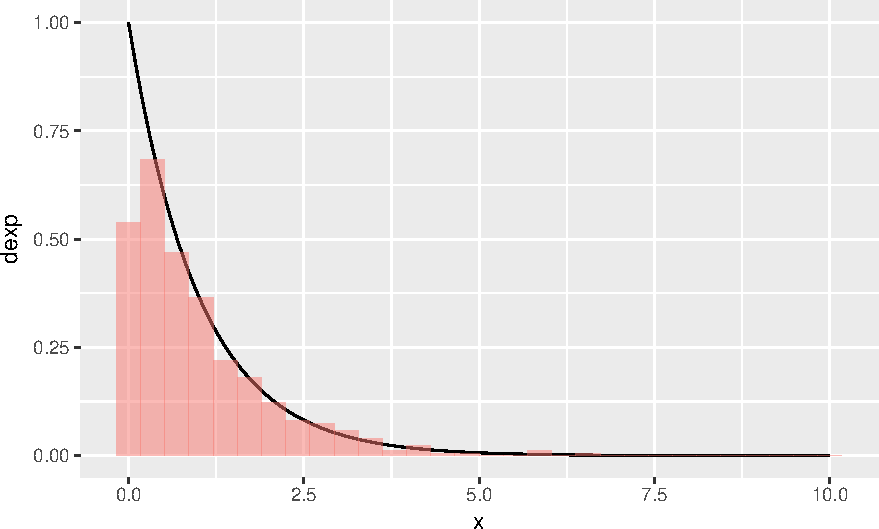
\includegraphics[width=0.7\linewidth]{statistical-computing_files/figure-latex/cdfexp-1} 

}

\caption{Inverse Transformation: Exp(1)}\label{fig:cdfexp}
\end{figure}

\hypertarget{discrete-case}{%
\subsection{Discrete case}\label{discrete-case}}

\begin{enumerate}
\def\labelenumi{\arabic{enumi}.}
\tightlist
\item
  For each \(i = 1, 2, \ldots, n\):

  \begin{enumerate}
  \def\labelenumii{\alph{enumii}.}
  \tightlist
  \item
    Generate \(u_i \sim unif(0, 1)\)
  \item
    Take \(x_i\) s.t. \(F_X(x_{i - 1}) < U \le F_X(x_i)\)
  \end{enumerate}
\end{enumerate}

Collect \(x_1, x_2, \ldots, x_n \sim F_X\).

\begin{Shaded}
\begin{Highlighting}[]
\NormalTok{pmf <-}
\StringTok{  }\KeywordTok{tibble}\NormalTok{(}
    \DataTypeTok{x =} \DecValTok{0}\OperatorTok{:}\DecValTok{4}\NormalTok{,}
    \DataTypeTok{p =} \KeywordTok{c}\NormalTok{(.}\DecValTok{1}\NormalTok{, }\FloatTok{.2}\NormalTok{, }\FloatTok{.2}\NormalTok{, }\FloatTok{.2}\NormalTok{, }\FloatTok{.3}\NormalTok{)}
\NormalTok{  )}
\end{Highlighting}
\end{Shaded}

\begin{longtable}[]{@{}lrrrrr@{}}
\caption{\label{tab:exdis}Example of a Discrete Random Variable}\tabularnewline
\toprule
\endhead
x & 0.0 & 1.0 & 2.0 & 3.0 & 4.0\tabularnewline
p & 0.1 & 0.2 & 0.2 & 0.2 & 0.3\tabularnewline
\bottomrule
\end{longtable}

\BeginKnitrBlock{example}[Discrete Random Variable]
\protect\hypertarget{exm:dismass}{}{\label{exm:dismass} \iffalse (Discrete Random Variable) \fi{} }Consider a discrete random variable \(X\) with a mass function as in Table \ref{tab:exdis}.
\EndKnitrBlock{example}

i.e.

\begin{figure}[H]

{\centering 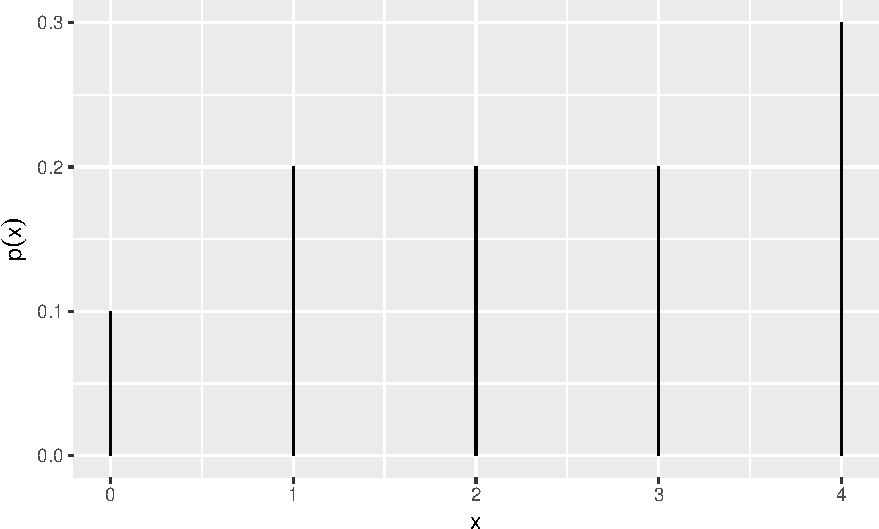
\includegraphics[width=0.7\linewidth]{statistical-computing_files/figure-latex/massfun-1} 

}

\caption{Probability Mass Function}\label{fig:massfun}
\end{figure}

Then we have the cdf

\begin{figure}[H]

{\centering 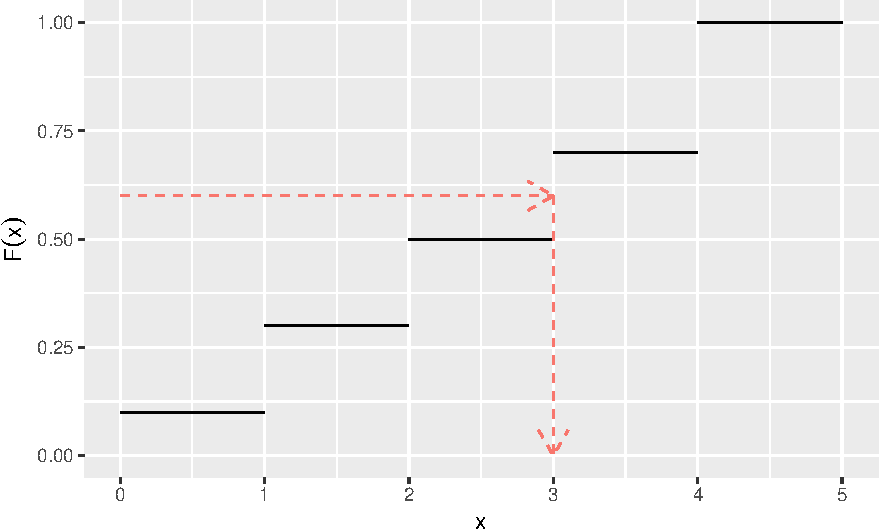
\includegraphics[width=0.7\linewidth]{statistical-computing_files/figure-latex/cdfun-1} 

}

\caption{CDF of the Discrete Random Variable: Illustration for discrete case}\label{fig:cdfun}
\end{figure}

Remembering the algorithm, we can implement \texttt{dplyr::case\_when()} here.

\begin{Shaded}
\begin{Highlighting}[]
\NormalTok{rcustom <-}\StringTok{ }\ControlFlowTok{function}\NormalTok{(n) \{}
  \KeywordTok{tibble}\NormalTok{(}\DataTypeTok{u =} \KeywordTok{runif}\NormalTok{(n)) }\OperatorTok\StringTok{ }
\StringTok{    }\KeywordTok{mutate}\NormalTok{(}
      \DataTypeTok{x =} \KeywordTok{case_when}\NormalTok{(}
\NormalTok{        u }\OperatorTok{>}\StringTok{ }\DecValTok{0} \OperatorTok{&}\StringTok{ }\NormalTok{u }\OperatorTok{<=}\StringTok{ }\FloatTok{.1} \OperatorTok{~}\StringTok{ }\DecValTok{0}\NormalTok{,}
\NormalTok{        u }\OperatorTok{>}\StringTok{ }\FloatTok{.1} \OperatorTok{&}\StringTok{ }\NormalTok{u }\OperatorTok{<=}\StringTok{ }\FloatTok{.3} \OperatorTok{~}\StringTok{ }\DecValTok{1}\NormalTok{,}
\NormalTok{        u }\OperatorTok{>}\StringTok{ }\FloatTok{.3} \OperatorTok{&}\StringTok{ }\NormalTok{u }\OperatorTok{<=}\StringTok{ }\FloatTok{.5} \OperatorTok{~}\StringTok{ }\DecValTok{2}\NormalTok{,}
\NormalTok{        u }\OperatorTok{>}\StringTok{ }\FloatTok{.5} \OperatorTok{&}\StringTok{ }\NormalTok{u }\OperatorTok{<=}\StringTok{ }\FloatTok{.7} \OperatorTok{~}\StringTok{ }\DecValTok{3}\NormalTok{,}
        \OtherTok{TRUE} \OperatorTok{~}\StringTok{ }\DecValTok{4}
\NormalTok{      )}
\NormalTok{    ) }\OperatorTok\StringTok{ }
\StringTok{    }\KeywordTok{select}\NormalTok{(x) }\OperatorTok\StringTok{ }
\StringTok{    }\KeywordTok{pull}\NormalTok{()}
\NormalTok{\}}
\end{Highlighting}
\end{Shaded}

\begin{Shaded}
\begin{Highlighting}[]
\KeywordTok{tibble}\NormalTok{(}
  \DataTypeTok{x =} \KeywordTok{rcustom}\NormalTok{(}\DecValTok{100}\NormalTok{)}
\NormalTok{) }\OperatorTok\StringTok{ }
\StringTok{  }\KeywordTok{ggplot}\NormalTok{(}\KeywordTok{aes}\NormalTok{(}\DataTypeTok{x =}\NormalTok{ x)) }\OperatorTok{+}
\StringTok{  }\KeywordTok{geom_histogram}\NormalTok{(}\KeywordTok{aes}\NormalTok{(}\DataTypeTok{y =}\NormalTok{ ..ndensity..), }\DataTypeTok{binwidth =} \FloatTok{.1}\NormalTok{)}
\end{Highlighting}
\end{Shaded}

\begin{figure}[H]

{\centering 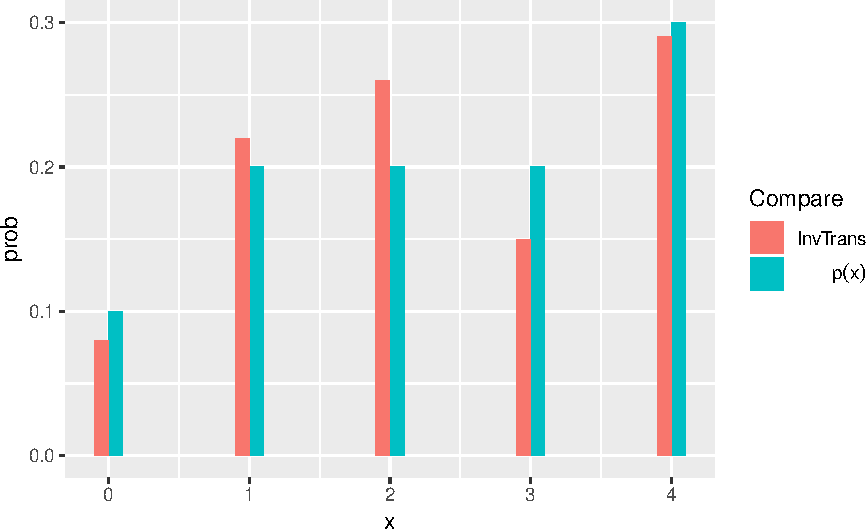
\includegraphics[width=0.7\linewidth]{statistical-computing_files/figure-latex/randmass-1} 

}

\caption{Generated discrete random numbers}\label{fig:randmass}
\end{figure}

See Figure \ref{fig:massfun} and \ref{fig:randmass}. Comparing the two, the result can be said okay.

\hypertarget{problems-with-inverse-transformation}{%
\subsection{Problems with inverse transformation}\label{problems-with-inverse-transformation}}

Examples \ref{exm:expon} and \ref{exm:dismass}. We could generate these random numbers because we aware of

\begin{enumerate}
\def\labelenumi{\arabic{enumi}.}
\tightlist
\item
  analytical \(F_X\)
\item
  \(F^{-1}\)
\end{enumerate}

In practice, however, not all distribution have analytical \(F\). Numerical computing might be possible, but it is not efficient. There are other approaches.

\hypertarget{the-acceptance-rejection-method}{%
\section{The Acceptance-Rejection Method}\label{the-acceptance-rejection-method}}

Acceptance-rejection method does not require analytical form of cdf. What we need is our \emph{target} density (or mass) function and \emph{proposal} density (or mass) function. Target function is what we want to generate. Propsal function is of any random variable that is \emph{easy to generate random numbers}. From this approach, we can generate any distribution while computation is not efficient.

\begin{longtable}[]{@{}cc@{}}
\toprule
pdf or pmf & target or proposal\tabularnewline
\midrule
\endhead
\(f\) & target\tabularnewline
\(g\) & proposal - easy to generate random numbers\tabularnewline
\bottomrule
\end{longtable}

First of all, \(g\) should satisfy that

\[spt f \subseteq spt g\]

Next, for some (pre-specified) \(c > 0\)

\[\forall x \in spt f : \frac{f(x)}{g(x)} \le c\]

\hypertarget{a-r-algorithm}{%
\subsection{A-R algorithm}\label{a-r-algorithm}}

For \(i = 1, \ldots, n\)

\begin{enumerate}
\def\labelenumi{\arabic{enumi}.}
\tightlist
\item
  \(Y \sim g(Y)\)
\item
  \(U \sim unif(0, 1) \perp\!\!\!\perp Y\)
\item
  Accept-Reject step

  \begin{enumerate}
  \def\labelenumii{\alph{enumii}.}
  \tightlist
  \item
    Accept: \(U \le \frac{f(Y)}{cg(Y)} \Rightarrow x_i = Y\)
  \item
    Reject: otherwise, go to step 1
  \end{enumerate}
\end{enumerate}

Collect \(x_1, x_2, \ldots, x_n \stackrel{iid}{\sim} f(x)\).

\hypertarget{efficiency}{%
\subsection{Efficiency}\label{efficiency}}

\begin{figure}[H]

{\centering 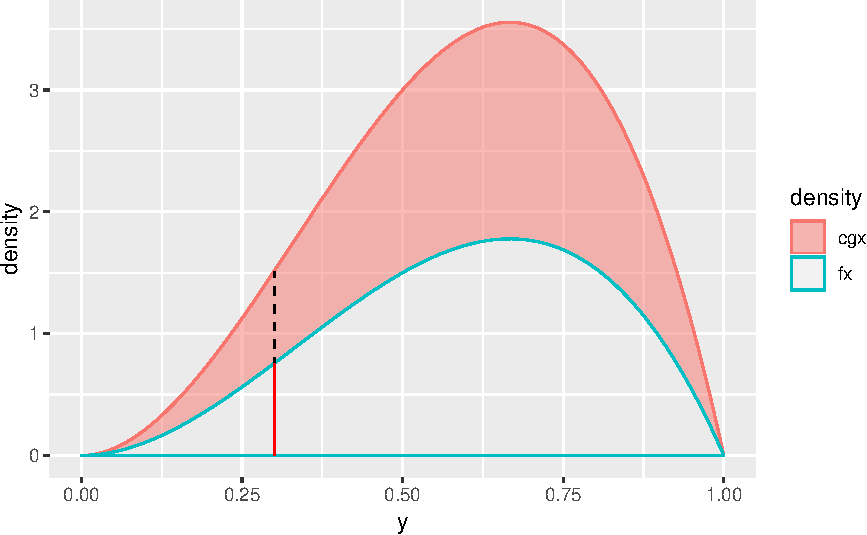
\includegraphics[width=0.7\linewidth]{statistical-computing_files/figure-latex/arprop-1} 

}

\caption{Property of AR method}\label{fig:arprop}
\end{figure}

See Figure \ref{fig:arprop}. This illustrates the motivation of A-R method. Lower one is \(f(x)\) and the upper one is \(cg(x)\) which covers \(f\). We can see that

\[0 < \frac{f(x)}{cg(x)} \le 1\]

The algorithm takes random number from \(Y \sim g\) in each recursive step \(i\), which is represented as a line in the figure. At this value, the algorithm accept \(Y\) as random number of \(f\) if

\[U \le \frac{f(Y)}{cg(Y)}\]

Suppose that we choose a point at random on a line drawn in the figure \ref{fig:arprop}. If we get the red line, we accept. Otherwise, we reject. In other words, the \emph{colored area is where we reject the given value}. The smaller the area is, the more efficient the algorithm will be.

\BeginKnitrBlock{proposition}[Properties of A-R Method]
\protect\hypertarget{prp:arnote}{}{\label{prp:arnote} \iffalse (Properties of A-R Method) \fi{} }\(\text{(1)}\: \frac{f(Y)}{cg(Y)} \perp\!\!\!\perp U\)

\(\text{(2)}\: 0 < \frac{f(x)}{cg(x)} \le 1\)

\(\text{(3)}\:\) Let \(N\) be the number of iterations needed to get an acceptance. Then

\[N \sim Geo(p) \quad \text{where}\: p \equiv P\bigg(U \le \frac{f(Y)}{cg(Y)}\bigg)\]

and so

\[
\begin{cases}
  P(N = n) = p(1 - p)^{n - 1}I_{\{1, 2, \ldots \}}(n) \\
  E(N) = \text{average number of iterations} = \frac{1}{p}
\end{cases}
\]

\(\text{(4)}\: X \sim Y \mid U \le \frac{f(Y)}{cg(Y)}\), i.e.

\[P\bigg(Y \le y \mid U \le \frac{f(Y)}{cg(Y)}\bigg) = F_X(y)\]
\EndKnitrBlock{proposition}

\BeginKnitrBlock{remark}[Efficiency]
\iffalse{} {Remark (Efficiency). } \fi{}Efficiency of the A-R method depends on \(p = P\bigg(U \le \frac{f(Y)}{cg(Y)}\bigg)\). In fact,

\[E(N) = \frac{1}{p} = c\]

The algorithm becomes efficient for small \(c\).
\EndKnitrBlock{remark}

\BeginKnitrBlock{proof}
\iffalse{} {Proof. } \fi{}Note that

\[P\bigg( U \le \frac{f(y)}{cg(y)}, Y = y \bigg) = P\bigg(Y \le \frac{g(y)}{cg(y)} \mid Y = y \bigg)P(Y = y)\]

Since \(U \sim unif(0, 1)\), \(P\bigg(Y \le \frac{g(y)}{cg(y)} \mid Y = y \bigg) = \frac{f(y)}{cg(y)}\).

By construction, \(P(Y = y) = g(y)\).

It follows that

\begin{equation*}
  \begin{split}
    p = P\bigg( U \le  \frac{f(y)}{cg(y)} \bigg) & = \int_{-\infty}^{\infty} P\bigg( U \le \frac{f(y)}{cg(y)}, Y = y \bigg) dy \\
    & = \int_{-\infty}^{\infty} \frac{f(y)}{cg(y)} g(y) dy \\
    & = \frac{1}{c} \int_{-\infty}^{\infty}f(y)dy \\
    & = \frac{1}{c}
  \end{split}
\end{equation*}

Hence,

\[E(N) = \frac{1}{p} = c\]

We can say that the method is efficient when the acceptance rate \(p\) is large, i.e.~\(c\) small.
\EndKnitrBlock{proof}

\BeginKnitrBlock{corollary}[Efficiency of A-R Method]
\protect\hypertarget{cor:argood}{}{\label{cor:argood} \iffalse (Efficiency of A-R Method) \fi{} }A-R method is efficient when

\(g(\cdot)\) is close to \(f(\cdot)\) and

have small \(c\).
\EndKnitrBlock{corollary}

\BeginKnitrBlock{corollary}[Choosing c]
\protect\hypertarget{cor:arc}{}{\label{cor:arc} \iffalse (Choosing c) \fi{} }To enhance the algorithm, we might choose \(c\) which satisfy

\[c = \max \bigg\{ \frac{f(x)}{g(x)} : x \in spt f \bigg\}\]
\EndKnitrBlock{corollary}

\hypertarget{examples}{%
\subsection{Examples}\label{examples}}

\BeginKnitrBlock{example}[Beta(a,b)]
\protect\hypertarget{exm:arbeta}{}{\label{exm:arbeta} \iffalse (Beta(a,b)) \fi{} }Let \(X \sim Beta(a, b)\). Then the pdf of \(X\) is given by

\[f(x) = \frac{1}{B(a, b)}x^{a - 1}(1 - x)^{b - 1}I_{(0, 1)}(x)\]
\EndKnitrBlock{example}

\BeginKnitrBlock{solution}[Generating Beta(a,b) with A-R method]
\iffalse{} {Solution (Generating Beta(a,b) with A-R method). } \fi{}Consider proposal density \(g(x) = I_{(0, 1)}(x)\), i.e.~\(unif(0, 1)\).

To determine the optimal \(c\) s.t.

\[c = \max \bigg\{ \frac{f(x)}{g(x)} : x \in (0, 1) \bigg\}\]

find the maximum of

\[\frac{f(x)}{g(x)} = \frac{1}{B(a, b)}x^{a - 1}(1 - x)^{b - 1}\]

Solve

\begin{equation*}
  \begin{split}
    \frac{d}{dx}\bigg(\frac{f(x)}{g(x)}\bigg) & = \frac{1}{B(a, b)}\Big( (a-1)x^{a-2}(1 - x)^{b - 1} - (b - 1)x^{a - 1}(1 - x)^{b - 2} \Big) \\
    & = \frac{x^{a - 2}(1 - x)^{b - 2}}{B(a, b)} \Big( (a - 1)(1 - x) - (b - 1)x \Big) \\
    & = \frac{x^{a - 2}(1 - x)^{b - 2}}{B(a, b)} \big( a - 1 - (a + b - 2)x \big) \quad = 0
  \end{split}
\end{equation*}

It follows that

\[\frac{f(x)}{g(x)} \le \frac{f(\frac{a - 1}{a + b - 2})}{g(\frac{a - 1}{a + b - 2})} = c\]

if \(\frac{a - 1}{a + b - 2} \neq 0, 1\)
\EndKnitrBlock{solution}

\begin{Shaded}
\begin{Highlighting}[]
\NormalTok{ar_beta <-}\StringTok{ }\ControlFlowTok{function}\NormalTok{(n, a, b) \{}
\NormalTok{  opt_x <-}\StringTok{ }\NormalTok{(a }\OperatorTok{-}\StringTok{ }\DecValTok{1}\NormalTok{) }\OperatorTok{/}\StringTok{ }\NormalTok{(a }\OperatorTok{+}\StringTok{ }\NormalTok{b }\OperatorTok{-}\StringTok{ }\DecValTok{2}\NormalTok{)}
\NormalTok{  opt_c <-}\StringTok{ }\KeywordTok{dbeta}\NormalTok{(opt_x, }\DataTypeTok{shape1 =}\NormalTok{ a, }\DataTypeTok{shape2 =}\NormalTok{ b) }\OperatorTok{/}\StringTok{ }\KeywordTok{dunif}\NormalTok{(opt_x)}
\NormalTok{  X <-}\StringTok{ }\OtherTok{NULL}
\NormalTok{  N <-}\StringTok{ }\DecValTok{0}
  \ControlFlowTok{while}\NormalTok{ (N }\OperatorTok{<=}\StringTok{ }\NormalTok{n) \{}
\NormalTok{    Y <-}\StringTok{ }\KeywordTok{runif}\NormalTok{(n)}
\NormalTok{    U <-}\StringTok{ }\KeywordTok{runif}\NormalTok{(n)}
\NormalTok{    X <-}\StringTok{ }\KeywordTok{c}\NormalTok{(X, Y[U }\OperatorTok{<=}\StringTok{ }\KeywordTok{dbeta}\NormalTok{(Y, }\DataTypeTok{shape1 =}\NormalTok{ a, }\DataTypeTok{shape2 =}\NormalTok{ b) }\OperatorTok{/}\StringTok{ }\NormalTok{opt_c])}
\NormalTok{    N <-}\StringTok{ }\KeywordTok{length}\NormalTok{(X)}
    \ControlFlowTok{if}\NormalTok{ ( N }\OperatorTok{>}\StringTok{ }\NormalTok{n ) X <-}\StringTok{ }\NormalTok{X[}\DecValTok{1}\OperatorTok{:}\NormalTok{n]}
\NormalTok{  \}}
\NormalTok{  X}
\NormalTok{\}}
\end{Highlighting}
\end{Shaded}

Now we try to compare this A-R function to \texttt{R} \texttt{rbeta} function.

\begin{Shaded}
\begin{Highlighting}[]
\NormalTok{gen_beta <-}
\StringTok{  }\KeywordTok{tibble}\NormalTok{(}
    \DataTypeTok{ar_rand =} \KeywordTok{ar_beta}\NormalTok{(}\DecValTok{1000}\NormalTok{, }\DecValTok{3}\NormalTok{, }\DecValTok{2}\NormalTok{),}
    \DataTypeTok{sam =} \KeywordTok{rbeta}\NormalTok{(}\DecValTok{1000}\NormalTok{, }\DecValTok{3}\NormalTok{, }\DecValTok{2}\NormalTok{)}
\NormalTok{  ) }\OperatorTok\StringTok{ }
\StringTok{  }\KeywordTok{gather}\NormalTok{(}\DataTypeTok{key =} \StringTok{"den"}\NormalTok{, }\DataTypeTok{value =} \StringTok{"value"}\NormalTok{)}
\end{Highlighting}
\end{Shaded}

\begin{Shaded}
\begin{Highlighting}[]
\KeywordTok{gg_curve}\NormalTok{(dbeta, }\DataTypeTok{from =} \DecValTok{0}\NormalTok{, }\DataTypeTok{to =} \DecValTok{1}\NormalTok{, }\DataTypeTok{args =} \KeywordTok{list}\NormalTok{(}\DataTypeTok{shape1 =} \DecValTok{3}\NormalTok{, }\DataTypeTok{shape2 =} \DecValTok{2}\NormalTok{)) }\OperatorTok{+}
\StringTok{  }\KeywordTok{geom_histogram}\NormalTok{(}
    \DataTypeTok{data =}\NormalTok{ gen_beta,}
    \KeywordTok{aes}\NormalTok{(}\DataTypeTok{x =}\NormalTok{ value, }\DataTypeTok{y =}\NormalTok{ ..density.., }\DataTypeTok{fill =}\NormalTok{ den),}
    \DataTypeTok{position =} \StringTok{"identity"}\NormalTok{,}
    \DataTypeTok{bins =} \DecValTok{30}\NormalTok{,}
    \DataTypeTok{alpha =} \FloatTok{.45}
\NormalTok{  ) }\OperatorTok{+}
\StringTok{  }\KeywordTok{scale_fill_discrete}\NormalTok{(}
    \DataTypeTok{name =} \StringTok{"random number"}\NormalTok{,}
    \DataTypeTok{labels =} \KeywordTok{c}\NormalTok{(}\StringTok{"AR"}\NormalTok{, }\StringTok{"rbeta"}\NormalTok{)}
\NormalTok{  )}
\end{Highlighting}
\end{Shaded}

\begin{figure}[H]

{\centering 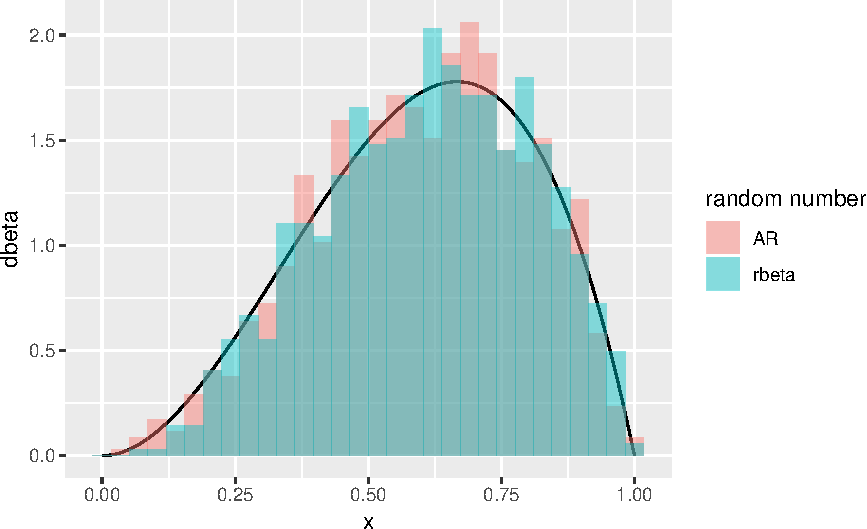
\includegraphics[width=0.7\linewidth]{statistical-computing_files/figure-latex/betahis-1} 

}

\caption{Beta(3,2) Random numbers from each function}\label{fig:betahis}
\end{figure}

In the Figure \ref{fig:betahis}, the both histograms are very close to the true density curve. To see more statistically, we can draw a Q-Q plot.

\begin{Shaded}
\begin{Highlighting}[]
\NormalTok{gen_beta }\OperatorTok\StringTok{ }
\StringTok{  }\KeywordTok{ggplot}\NormalTok{(}\KeywordTok{aes}\NormalTok{(}\DataTypeTok{sample =}\NormalTok{ value)) }\OperatorTok{+}
\StringTok{  }\KeywordTok{stat_qq_line}\NormalTok{(}
    \DataTypeTok{distribution =}\NormalTok{ stats}\OperatorTok{::}\NormalTok{qbeta,}
    \DataTypeTok{dparams =} \KeywordTok{list}\NormalTok{(}\DataTypeTok{shape1 =} \DecValTok{3}\NormalTok{, }\DataTypeTok{shape2 =} \DecValTok{2}\NormalTok{),}
    \DataTypeTok{col =} \KeywordTok{I}\NormalTok{(}\StringTok{"grey70"}\NormalTok{),}
    \DataTypeTok{size =} \FloatTok{3.5}
\NormalTok{  ) }\OperatorTok{+}
\StringTok{  }\KeywordTok{stat_qq}\NormalTok{(}
    \KeywordTok{aes}\NormalTok{(}\DataTypeTok{colour =}\NormalTok{ den),}
    \DataTypeTok{distribution =}\NormalTok{ stats}\OperatorTok{::}\NormalTok{qbeta,}
    \DataTypeTok{dparams =} \KeywordTok{list}\NormalTok{(}\DataTypeTok{shape1 =} \DecValTok{3}\NormalTok{, }\DataTypeTok{shape2 =} \DecValTok{2}\NormalTok{)}
\NormalTok{  ) }\OperatorTok{+}
\StringTok{  }\KeywordTok{scale_colour_discrete}\NormalTok{(}
    \DataTypeTok{name =} \StringTok{"random number"}\NormalTok{,}
    \DataTypeTok{labels =} \KeywordTok{c}\NormalTok{(}\StringTok{"AR"}\NormalTok{, }\StringTok{"rbeta"}\NormalTok{)}
\NormalTok{  )}
\end{Highlighting}
\end{Shaded}

\begin{figure}[H]

{\centering 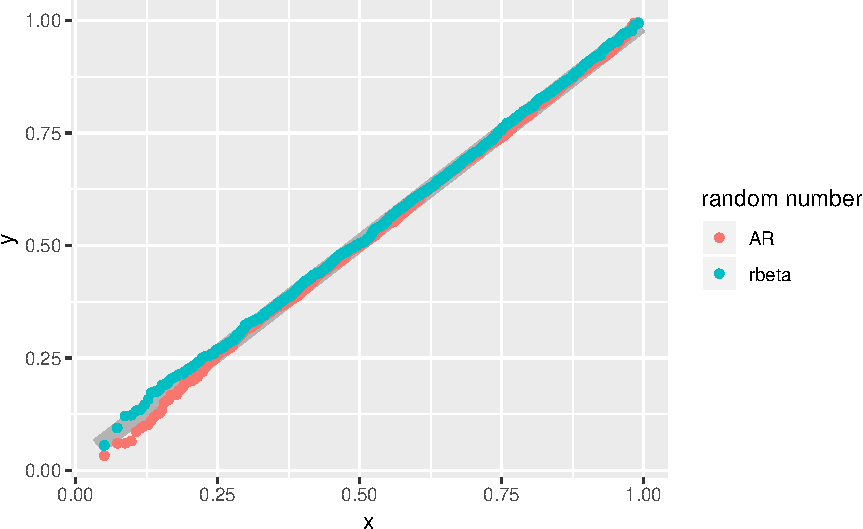
\includegraphics[width=0.7\linewidth]{statistical-computing_files/figure-latex/betaqq-1} 

}

\caption{Q-Q plot for Beta(3,2) random numbers}\label{fig:betaqq}
\end{figure}

See Figure \ref{fig:betaqq}. We have got series of numbers that are sticked to the beta distribution line.

\BeginKnitrBlock{example}[A-R Method for Discrete case]
\protect\hypertarget{exm:ardiscrete}{}{\label{exm:ardiscrete} \iffalse (A-R Method for Discrete case) \fi{} }A-R method can be also implemented to discrete case such as Example \ref{exm:dismass}.
\EndKnitrBlock{example}

\begin{longtable}[]{@{}lrrrrr@{}}
\caption{\label{tab:exdis2}Example of a Discrete Random Variable}\tabularnewline
\toprule
\endhead
x & 0.0 & 1.0 & 2.0 & 3.0 & 4.0\tabularnewline
p & 0.1 & 0.2 & 0.2 & 0.2 & 0.3\tabularnewline
\bottomrule
\end{longtable}

\BeginKnitrBlock{solution}[Generating discrete random numbers using A-R methods]
\iffalse{} {Solution (Generating discrete random numbers using A-R methods). } \fi{}Consider proposal \(g(x) \sim \text{Discrete unif}(0, 1, 2, 3, 4)\), i.e.

\[g(0) = g(1) = \cdots = g(4) = 0.2\]

Then we set

\[c = \max\bigg\{ \frac{p(x)}{g(x)} : x = 0, \ldots, 4 \bigg\} = \max\Big\{ 0.5, 1, 1.5 \Big\} = 1.5\]
\EndKnitrBlock{solution}

\hypertarget{transfomation-methods}{%
\section{Transfomation Methods}\label{transfomation-methods}}

\hypertarget{sums-and-mixtures}{%
\section{Sums and Mixtures}\label{sums-and-mixtures}}

\hypertarget{sums}{%
\subsection{Sums}\label{sums}}

\hypertarget{convolutions-and-mixtures}{%
\subsection{Convolutions and mixtures}\label{convolutions-and-mixtures}}

\begin{Shaded}
\begin{Highlighting}[]
\KeywordTok{library}\NormalTok{(foreach)}
\end{Highlighting}
\end{Shaded}

\begin{Shaded}
\begin{Highlighting}[]
\NormalTok{mix_norm <-}\StringTok{ }\ControlFlowTok{function}\NormalTok{(n, p1, mean1, sd1, mean2, sd2) \{}
\NormalTok{  x1 <-}\StringTok{ }\KeywordTok{rnorm}\NormalTok{(n, }\DataTypeTok{mean =}\NormalTok{ mean1, }\DataTypeTok{sd =}\NormalTok{ sd1)}
\NormalTok{  x2 <-}\StringTok{ }\KeywordTok{rnorm}\NormalTok{(n, }\DataTypeTok{mean =}\NormalTok{ mean2, }\DataTypeTok{sd =}\NormalTok{ sd2)}
\NormalTok{  k <-}\StringTok{ }\KeywordTok{as.integer}\NormalTok{(}\KeywordTok{runif}\NormalTok{(n) }\OperatorTok{>}\StringTok{ }\NormalTok{p1)}
\NormalTok{  k }\OperatorTok{*}\StringTok{ }\NormalTok{x1 }\OperatorTok{+}\StringTok{ }\NormalTok{(}\DecValTok{1} \OperatorTok{-}\StringTok{ }\NormalTok{k) }\OperatorTok{*}\StringTok{ }\NormalTok{x2}
\NormalTok{\}}
\end{Highlighting}
\end{Shaded}

\begin{Shaded}
\begin{Highlighting}[]
\NormalTok{mixture <-}
\StringTok{  }\KeywordTok{foreach}\NormalTok{(}\DataTypeTok{p1 =} \DecValTok{0}\OperatorTok{:}\DecValTok{10} \OperatorTok{/}\StringTok{ }\DecValTok{10}\NormalTok{, }\DataTypeTok{.combine =}\NormalTok{ bind_rows) }\OperatorTok\StringTok{ }\NormalTok{\{}
    \KeywordTok{tibble}\NormalTok{(}
      \DataTypeTok{value =} \KeywordTok{mix_norm}\NormalTok{(}\DataTypeTok{n =} \DecValTok{1000}\NormalTok{, }\DataTypeTok{p1 =}\NormalTok{ p1, }\DataTypeTok{mean1 =} \DecValTok{0}\NormalTok{, }\DataTypeTok{sd1 =} \DecValTok{1}\NormalTok{, }\DataTypeTok{mean2 =} \DecValTok{3}\NormalTok{, }\DataTypeTok{sd2 =} \DecValTok{1}\NormalTok{),}
      \DataTypeTok{key =} \KeywordTok{rep}\NormalTok{(p1, }\DecValTok{1000}\NormalTok{)}
\NormalTok{    )}
\NormalTok{  \}}
\end{Highlighting}
\end{Shaded}

\begin{Shaded}
\begin{Highlighting}[]
\NormalTok{mixture }\OperatorTok\StringTok{ }
\StringTok{  }\KeywordTok{ggplot}\NormalTok{(}\KeywordTok{aes}\NormalTok{(}\DataTypeTok{x =}\NormalTok{ value, }\DataTypeTok{colour =} \KeywordTok{factor}\NormalTok{(key))) }\OperatorTok{+}
\StringTok{  }\KeywordTok{stat_density}\NormalTok{(}\DataTypeTok{geom =} \StringTok{"line"}\NormalTok{, }\DataTypeTok{position =} \StringTok{"identity"}\NormalTok{) }\OperatorTok{+}
\StringTok{  }\KeywordTok{scale_colour_discrete}\NormalTok{(}
    \DataTypeTok{name =} \KeywordTok{expression}\NormalTok{(p[}\DecValTok{1}\NormalTok{]),}
    \DataTypeTok{labels =} \DecValTok{0}\OperatorTok{:}\DecValTok{10} \OperatorTok{/}\StringTok{ }\DecValTok{10}
\NormalTok{  ) }\OperatorTok{+}
\StringTok{  }\KeywordTok{xlab}\NormalTok{(}\StringTok{"x"}\NormalTok{)}
\end{Highlighting}
\end{Shaded}

\begin{center}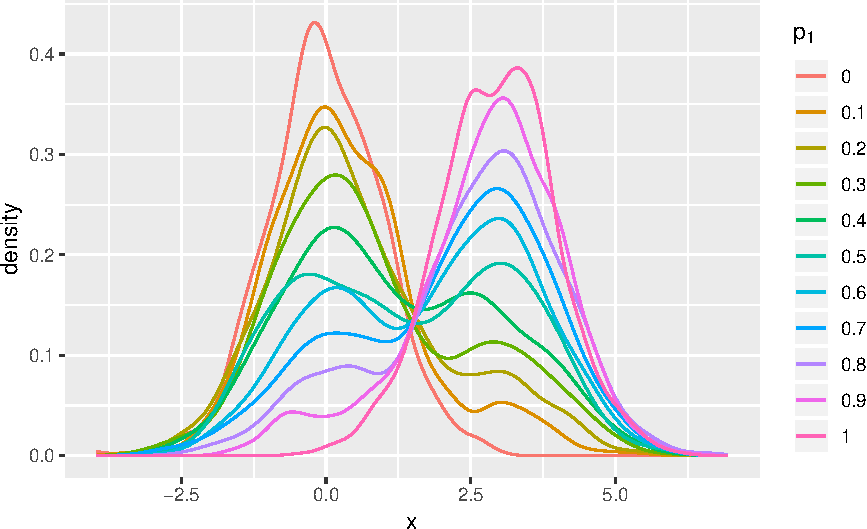
\includegraphics[width=0.7\linewidth]{statistical-computing_files/figure-latex/unnamed-chunk-20-1} \end{center}

\hypertarget{multivariate-normal-random-vector}{%
\section{Multivariate Normal Random Vector}\label{multivariate-normal-random-vector}}

\hypertarget{stochastic-processes}{%
\section{Stochastic Processes}\label{stochastic-processes}}

\hypertarget{homogeneous-poisson-process}{%
\subsection{Homogeneous poisson process}\label{homogeneous-poisson-process}}

\hypertarget{nonhomogeneous-poisson-process}{%
\subsection{Nonhomogeneous poisson process}\label{nonhomogeneous-poisson-process}}

\hypertarget{symmetric-random-walk}{%
\subsection{Symmetric random walk}\label{symmetric-random-walk}}

\hypertarget{mcint}{%
\chapter{Monte Carlo Integration and Variance Reduction}\label{mcint}}

\hypertarget{monte-carlo-integration}{%
\section{Monte Carlo Integration}\label{monte-carlo-integration}}

Consider integration problem of a integrable function \(g(x)\). We want to compute

\[\int_a^b g(x) dx\]

For instance, \(g(x) = e^{x^2}\)

\BeginKnitrBlock{example}
\protect\hypertarget{exm:mcex}{}{\label{exm:mcex} }\[\int_0^1 e^{x^2} dx\]
\EndKnitrBlock{example}

It seems tricky to compute the integral \ref{exm:mcex} analytically even though possible. So we implement \emph{simulation} concept here, based on the following theorems.

\BeginKnitrBlock{theorem}[Weak Law of Large Numbers]
\protect\hypertarget{thm:wlaw}{}{\label{thm:wlaw} \iffalse (Weak Law of Large Numbers) \fi{} }Suppose that \(X_1, \ldots, X_n \iid (\mu, \sigma^2 < \infty)\). Then

\[\frac{1}{n}\sum_{i = 1}^n X_i \stackrel{p}{\rightarrow} \mu\]

Let \(g\) be a measurable function. Then

\[\frac{1}{n}\sum_{i = 1}^n g(X_i) \stackrel{p}{\rightarrow} g(\mu)\]
\EndKnitrBlock{theorem}

\BeginKnitrBlock{theorem}[Strong Law of Large Numbers]
\protect\hypertarget{thm:slaw}{}{\label{thm:slaw} \iffalse (Strong Law of Large Numbers) \fi{} }Suppose that \(X_1, \ldots, X_n \iid (\mu, \sigma^2 < \infty)\). Then

\[\frac{1}{n}\sum_{i = 1}^n X_i \stackrel{a.s.}{\rightarrow} \mu\]

Let \(g\) be a measurable function. Then

\[\frac{1}{n}\sum_{i = 1}^n g(X_i) \stackrel{a.s.}{\rightarrow} g(\mu)\]
\EndKnitrBlock{theorem}

\hypertarget{simple-monte-carlo-estimator}{%
\subsection{Simple Monte Carlo estimator}\label{simple-monte-carlo-estimator}}

Suppose that we have a distribution \(f(x)\). Consider

\begin{equation}
  I \equiv \int_{spt f} g(x)f(x) dx
  \label{eq:muint}
\end{equation}

By \emph{the Strong law of large numbers} \ref{thm:slaw},

\[\frac{1}{n}\sum_{i = 1}^n g(X_i) \stackrel{a.s.}{\rightarrow} E\Big[g(X)\Big] = I\]

\BeginKnitrBlock{theorem}[Monte Carlo Integration]
\protect\hypertarget{thm:mcint}{}{\label{thm:mcint} \iffalse (Monte Carlo Integration) \fi{} }Consider integration \eqref{eq:muint}. This can be approximated via appropriate pdf \(f(x)\) by

\[\hat\theta_M = \frac{1}{M} \sum_{i = 1}^M g(X_i)\]
\EndKnitrBlock{theorem}

Go back to Example \ref{exm:mcex}.

\BeginKnitrBlock{solution}
\iffalse{} {Solution. } \fi{}\begin{equation*}
  \begin{split}
    I & \equiv \int_0^1 e^{x^2} dx \\
    & = \int_0^1 \frac{e^{x^2}}{f(x)}f(x) dx \qquad f(x) = \frac{e^x}{e - 1} : pdf \\
    & = \int_0^1 (e - 1)\exp(x^2 - x)f(x)dx \\
    & \approx \frac{1}{M} \sum_{m = 1}^M (e - 1)\exp(X_m^2 - X_m)
  \end{split}
\end{equation*}

Then generate \(X_1, \ldots, X_M \sim f(x)\).

Let \(F(X_1), \ldots, F(X_M) \iid unif(0, 1)\) where

\[F(x) = \int_0^x f(t)dt = \frac{e^x - 1}{e - 1}\]

i.e.~\(U_1 = \frac{e^{X_1} - 1}{e - 1}, \ldots, U_M = \frac{e^{X_M} - 1}{e - 1} \iid unif(0, 1)\). Hence,

\[X_m = \ln (1 + (e - 1) U_m)\]
\EndKnitrBlock{solution}

i.e.

\begin{enumerate}
\def\labelenumi{\arabic{enumi}.}
\tightlist
\item
  \(u_1, \ldots, u_M \iid unif(0,1)\)
\item
  \(x_i = \ln (1 + (e - 1) u_i)\)
\end{enumerate}

\begin{Shaded}
\begin{Highlighting}[]
\NormalTok{x <-}\StringTok{ }\KeywordTok{log}\NormalTok{(}\DecValTok{1} \OperatorTok{+}\StringTok{ }\NormalTok{(}\KeywordTok{exp}\NormalTok{(}\DecValTok{1}\NormalTok{) }\OperatorTok{-}\StringTok{ }\DecValTok{1}\NormalTok{) }\OperatorTok{*}\StringTok{ }\KeywordTok{runif}\NormalTok{(}\DecValTok{10000}\NormalTok{))}
\KeywordTok{mean}\NormalTok{((}\KeywordTok{exp}\NormalTok{(}\DecValTok{1}\NormalTok{) }\OperatorTok{-}\StringTok{ }\DecValTok{1}\NormalTok{) }\OperatorTok{*}\StringTok{ }\KeywordTok{exp}\NormalTok{(x}\OperatorTok{^}\DecValTok{2} \OperatorTok{-}\StringTok{ }\NormalTok{x))}
\NormalTok{[}\DecValTok{1}\NormalTok{] }\FloatTok{1.46}
\end{Highlighting}
\end{Shaded}

This method is also helpful solving high-dimensional problem.

\BeginKnitrBlock{example}[Higher dimensional problem]
\protect\hypertarget{exm:mcex2}{}{\label{exm:mcex2} \iffalse (Higher dimensional problem) \fi{} }\[\int_0^1 \int_0^1 e^{(x_1 + x_2)^2} dx_1 dx_2\]
\EndKnitrBlock{example}

\BeginKnitrBlock{solution}
\iffalse{} {Solution. } \fi{}\begin{equation*}
  \begin{split}
    I & \equiv \int_0^1 \int_0^1 e^{(x_1 + x_2)^2} dx_1 dx_2 \\
    & = \int_0^1\int_0^1 \frac{e^{(x_1 + x_2)^2}}{f(x_1, x_2)}f(x_1, x_2) dx_1dx_2 \qquad f(x) = \frac{e^{(x_1 + x_2)}}{(e - 1)^2} = \frac{e^{x_1}}{e - 1} + \frac{e^{x_2}}{e - 1} \\
    & = \int_0^1\int_0^1 (e - 1)^2\exp((x_1 + x_2)^2 - x_1 - x_2)f(x_1, x_2)dx_1dx_2 \\
    & \approx \frac{1}{M} \sum_{m = 1}^M (e - 1)^2\exp((X_{1m} + X_{2m})^2 - X_{1m} - X_{2m})
  \end{split}
\end{equation*}
\EndKnitrBlock{solution}

Hence,

\begin{enumerate}
\def\labelenumi{\arabic{enumi}.}
\tightlist
\item
  \(u_{1m}, u_{2m} \sim unif(0,1), \quad m = 1, \ldots, M\)
\item
  \(x_{jm} = \ln(1 + (e - 1)u_{jm}), \quad j = 1, 2, \quad m = 1, \ldots, M\)
\end{enumerate}

\begin{Shaded}
\begin{Highlighting}[]
\KeywordTok{tibble}\NormalTok{(}
  \DataTypeTok{x1 =} \KeywordTok{log}\NormalTok{(}\DecValTok{1} \OperatorTok{+}\StringTok{ }\NormalTok{(}\KeywordTok{exp}\NormalTok{(}\DecValTok{1}\NormalTok{) }\OperatorTok{-}\StringTok{ }\DecValTok{1}\NormalTok{) }\OperatorTok{*}\StringTok{ }\KeywordTok{runif}\NormalTok{(}\DecValTok{10000}\NormalTok{)),}
  \DataTypeTok{x2 =} \KeywordTok{log}\NormalTok{(}\DecValTok{1} \OperatorTok{+}\StringTok{ }\NormalTok{(}\KeywordTok{exp}\NormalTok{(}\DecValTok{1}\NormalTok{) }\OperatorTok{-}\StringTok{ }\DecValTok{1}\NormalTok{) }\OperatorTok{*}\StringTok{ }\KeywordTok{runif}\NormalTok{(}\DecValTok{10000}\NormalTok{))}
\NormalTok{) }\OperatorTok\StringTok{ }
\StringTok{  }\KeywordTok{summarise}\NormalTok{(}\DataTypeTok{int =} \KeywordTok{mean}\NormalTok{((}\KeywordTok{exp}\NormalTok{(}\DecValTok{1}\NormalTok{) }\OperatorTok{-}\StringTok{ }\DecValTok{1}\NormalTok{)}\OperatorTok{^}\DecValTok{2} \OperatorTok{*}\StringTok{ }\KeywordTok{exp}\NormalTok{((x1 }\OperatorTok{+}\StringTok{ }\NormalTok{x2)}\OperatorTok{^}\DecValTok{2} \OperatorTok{-}\StringTok{ }\NormalTok{x1 }\OperatorTok{-}\StringTok{ }\NormalTok{x2)))}
\CommentTok{# A tibble: 1 x 1}
\NormalTok{    int}
  \OperatorTok{<}\NormalTok{dbl}\OperatorTok{>}
\DecValTok{1}  \FloatTok{4.95}
\end{Highlighting}
\end{Shaded}

\hypertarget{standard-error}{%
\subsection{Standard error}\label{standard-error}}

\hypertarget{variance-and-efficiency}{%
\section{Variance and Efficiency}\label{variance-and-efficiency}}

\hypertarget{variance}{%
\subsection{Variance}\label{variance}}

\hypertarget{efficiency-1}{%
\subsection{Efficiency}\label{efficiency-1}}

\hypertarget{variance-reduction}{%
\section{Variance Reduction}\label{variance-reduction}}

\hypertarget{antithetic-variables}{%
\section{Antithetic Variables}\label{antithetic-variables}}

\hypertarget{control-variates}{%
\section{Control Variates}\label{control-variates}}

\hypertarget{importance-sampling}{%
\section{Importance Sampling}\label{importance-sampling}}

\bibliography{book.bib,packages.bib}


\end{document}
